\documentclass[12pt]{article}

\usepackage[T2A]{fontenc}
\usepackage[utf8]{inputenc}
\usepackage[english, russian]{babel}

\usepackage[letterpaper,top=2cm,bottom=2cm,left=1.5cm,right=1.5cm,marginparwidth=1.75cm]{geometry}
\usepackage{float}
%\usepackage[stable]{footmisc}

\usepackage{amsmath,amssymb}
\usepackage{graphicx}
\usepackage[colorlinks=true, allcolors=blue]{hyperref}
\hypersetup{unicode=true}
\usepackage{url}
\usepackage{longtable,booktabs,array}
\usepackage{tablefootnote}
\usepackage{circuitikz}
\usetikzlibrary{fit}

\title{Лабораторная работа № 4 \\
``Ультразвуковой дальномер'' \\
\large Сенсоры и сенсорные системы}

\begin{document}
\maketitle
\tableofcontents
\begin{abstract}
    Применение ультразвука для измерения расстояний. Устройство и принцип работы ультразвукового дальномера. Фильтрация измерений.
\end{abstract}

\section{Цель работы}
Изучить принципы работы ультразвукового дальномера, оценить их возможности и ограничения, провести измерения и анализ результатов для различных объектов и условий.

\section{Теория}
\textbf{Ультразвуковой дальномер (сонар)} - это устройство, которое использует ультразвуковые волны для измерения расстояний до объектов или точек. 

\textbf{Ультразвуковые волны (УЗ волны)} - механические акустические волны, частота которых лежит за пределами слышимости человеческого уха - 20 кГц. Однако сигналы этих частот воспринимаются некоторыми животными: собаками, кошками, грызунами и насекомыми.

Ультразвуковые дальномеры широко применяются в различных областях, включая промышленность, автоматизацию, робототехнику, медицину и беспилотный транспорт.

Задачи, решаемые с их помощью:
\begin{itemize}
	\item предотвращение столкновений и обеспечение обхода пре-
	пятствий,
	\item картографирование окружающего пространства,
	\item распознавание объектов.
\end{itemize}

Широкое распространение сонаров объясняется их низкой стоимостью, небольшим весом и энергопотреблением, простотой обработки сигналов.

\subsection{Принцип действия}
 Принцип работы ультразвукового дальномера основан на измерении времени, за которое ультразвуковой сигнал, выпущенный излучателем, достигает объекта и возвращается к приемнику (эффект эха). Устройство измеряет время возврата сигнала и на основе скорости распространения ультразвука вычисляет расстояние до объекта. 
 
 Существует различные модификации ультразвуковых дальномеров, однако все они основаны на измерении времени, которое требуется для прохождения отраженного звука. Иначе говоря, датчик генерирует звуковой сигнал в определенном направлении, затем принимает отраженное эхо и рассчитывает время, которое звуку требуется для прохождения от датчика до препятствия и обратно (см.~рис. \ref{fig:screenshot001}).

\begin{figure}[H]
	\centering
	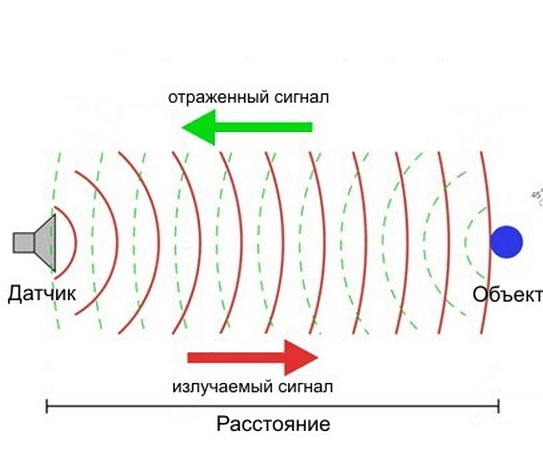
\includegraphics[width=0.7\linewidth]{images/screenshot001}
	\caption{Принцип работы ультразвукового дальномера}
	\label{fig:screenshot001}
\end{figure}

Расстояние до объекта \(L\) можно определить по скорости ультразвуковых волн:
\[s=\frac{vt}{2},\]
где \(v\) - скорость звука, которая отличается для различных сред. Она зависит в основном от плотности среды, в которой звук распространяется. Для воздуха при обычной температуре и плотности скорость звука составляет \(v=343 \text{ м/с}\);\\
\(t\) - время пролета ультразвуковой волны

\subsection{Источник ультразвука}
В воздушной среде используются частоты 30–100 кГц. В излучателях этих колебаний применяются электростатические, пьезоэлектрические, а так же магнитострикционные преобразователи электрического сигнала в ультразвук. Приемники устроены по принципу обратимых электроакустических преобразователей такого же принципа действия. Наибольшее распространение в приемниках и передатчиках получил прямой и обратный пьезоэффекты. Один и тот же обратимый преобразователь может использоваться и на излучение и на прием путем циклического переключения режима работы.

Возбуждение и прием УЗ-волн в используемом датчике осуществляется пьезоэлектрическим способом. Пьезоэлектрический материал обладает свойством, что под действием приложенного к нему механического воздействия на его поверхности возникают электрические заряды. Это называет прямой пьезоэлектрический эффект. Обратный ему происходит в случае, когда на приложенной электрическое напряжение материал реагирует изменением своей формы. Прямой эффект используется для измерений, обратный для генерации УЗ-волн. На рис.~\ref{fig:screenshot002}А показана типовая схема ультразвукового преобразователя, а на рис.~\ref{fig:screenshot002}Б его внешний вид и устройство

\begin{figure}[H]
	\centering
	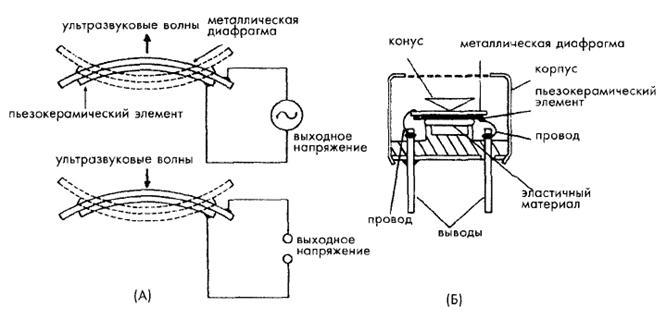
\includegraphics[width=0.7\linewidth]{images/screenshot002}
	\caption{Устройство пьезоэлектрического преобразователя}
	\label{fig:screenshot002}
\end{figure}


\subsection{УЗ дальномер HC-SR04}




\end{document}